%\documentclass[wcp,gray]{jmlr} % test grayscale version
\documentclass[wcp]{jmlr}

% The following packages will be automatically loaded:
% amsmath, amssymb, natbib, graphicx, url, algorithm2e

%\usepackage{rotating}% for sideways figures and tables
\usepackage{longtable}% for long tables

% The booktabs package is used by this sample document
% (it provides \toprule, \midrule and \bottomrule).
% Remove the next line if you don't require it.
\usepackage{booktabs}
% The siunitx package is used by this sample document
% to align numbers in a column by their decimal point.
% Remove the next line if you don't require it.
%\usepackage[load-configurations=version-1]{siunitx} % newer version
%\usepackage{siunitx}
%\usepackage{natbib}

% Do not comment the following commands:
\pagenumbering{gobble}
%\newenvironment{conditions}
%  {\par\vspace{\abovedisplayskip}\noindent\begin{tabular} {>{$}l<{$} @{${}={}$} l}}
%{\end{tabular}\par\vspace{\belowdisplayskip}}

\newcommand{\cs}[1]{\texttt{\char`\\#1}}
\makeatletter
\let\Ginclude@graphics\@org@Ginclude@graphics 
\makeatother

\jmlrvolume{}
\jmlryear{2022}
\jmlrworkshop{ACML 2022}

\title[Topological Framework for Activation function in DNN]{Design of Activation Function Using Topological Framework  in Deep Neural Networks}

 % Use \Name{Author Name} to specify the name.
 % If the surname contains spaces, enclose the surname
 % in braces, e.g. \Name{John {Smith Jones}} similarly
 % if the name has a "von" part, e.g \Name{Jane {de Winter}}.
 % If the first letter in the forenames is a diacritic
 % enclose the diacritic in braces, e.g. \Name{{\'E}louise Smith}

 % Two authors with the same address
 % \author{\Name{Author Name1} \Email{abc@sample.com}\and
 %  \Name{Author Name2} \Email{xyz@sample.com}\\
 %  \addr Address}

 % Three or more authors with the same address:
 % \author{\Name{Author Name1} \Email{an1@sample.com}\\
 %  \Name{Author Name2} \Email{an2@sample.com}\\
 %  \Name{Author Name3} \Email{an3@sample.com}\\
 %  \Name{Author Name4} \Email{an4@sample.com}\\
 %  \Name{Author Name5} \Email{an5@sample.com}\\
 %  \Name{Author Name6} \Email{an6@sample.com}\\
 %  \Name{Author Name7} \Email{an7@sample.com}\\
 %  \Name{Author Name8} \Email{an8@sample.com}\\
 %  \Name{Author Name9} \Email{an9@sample.com}\\
 %  \Name{Author Name10} \Email{an10@sample.com}\\
 %  \Name{Author Name11} \Email{an11@sample.com}\\
 %  \Name{Author Name12} \Email{an12@sample.com}\\
 %  \Name{Author Name13} \Email{an13@sample.com}\\
 %  \Name{Author Name14} \Email{an14@sample.com}\\
 %  \addr Address}

 % Authors with different addresses:
  \author{\Name{Author Name1} \Email{abc@sample.com}\\
  \addr Address 1
  \AND
  \Name{Author Name2} \Email{xyz@sample.com}\\
  \addr Address 2
 }

\editors{Emtiyaz Khan and Mehmet Gonen}

\begin{document}

\maketitle

\begin{abstract}
Success of deep neural networks in diverse tasks across domains of computer vision, speech recognition and natural language processing, has necessitated understanding the dynamics of training process and also working of trained models. For classification tasks, one of the main requirements of the layer transfer function is to transform data such that only information required for classification is preserved and all other information is discarded.  Further the data should be transformed such that samples belonging to a single class should come closer in the transformed space which will help in drawing a clear decision boundary across classes. This enforces the need for topological simplification of the point cloud data set formed using samples from each class. We analyze the topological transformation of the space of training samples as it gets transformed by each successive layer during training, by changing the activation function. The impact of changing activation function on the convergence during training is reported for the task of binary classification.  A novel activation function aimed at faster convergence for classification tasks is proposed.  Here, Betti numbers are used to quantify topological complexity of data. Results of experiments on popular synthetic binary classification datasets with large Betti numbers (>150) using MLPs are reported. Results show that the proposed activation function results in faster convergence requiring fewer epochs by a factor of 1.5  to 2, since Betti numbers reduce faster across layers with the proposed activation function. The proposed methodology was verified on benchmark image datasets: fashion MNIST, CIFAR-10 and cat-vs-dog images, using CNNs.
\end{abstract}
\begin{keywords}
Training Convergence; Activation function; Topological Data Analysis; Betti Numbers
\end{keywords}

\section{Introduction}

Deep neural networks have become the default choice for solving many  complex tasks across several domains \cite{alexnet, yolo, chen2017deeplab, ronneberger2015u}. This is mainly because: 1) many tasks in domains such as computer vision, speech analysis and NLP, involve high dimensional datasets for which a complex model is required 2)for tasks performed by humans, which they acquired by birth, it is not well now how humans perform the task and what features they use. Deep neural networks, originally inspired by biological neural networks in cat’s, is computing the features in a hierarchical fashion.

However, choosing the right architecture (like the  selection  of hyper parameters activation function, number of layers and number of units per layer)  for a specific task is mostly based on 1) trial and error or 2) previous empirical results of tasks of similar complexity. The transfer function of each layer and the entire neural network is just treated as a complex, unknown and nonlinear function parameterized by weights and biases.

In this study,  we investigate some of the  desired characteristics a neural network architecture should have for solving a classification task. We derive our results based on the topology of the space of training data and how this topology changes as data is transformed by each layer.

Topology is a field of mathematics that studies the shape of objects and associated invariances like connectedness, number of holes of different dimensions etc. \cite{betti_number}. It is observed that many real datasets when viewed as point cloud dataset in a high dimensional space follow  certain topology. For example the study  in \cite{carlsson2009topology} shows that the image patches obtained from natural images follow the topology of a Klein bottle \cite{klein_bottle}.

Topological data analysis\cite{carlsson2009topology, chazal2021introduction} uses topological tools, like persistent homology \cite{edelsbrunner2008persistent}, for analyzing point cloud dataset in order to identify and characterize underlying structures in a dataset.

In their recent study, \cite{naitzat2020topology}  uses Betti numbers \cite{betti_number} to quantify topological complexity. In their study, they make the following important observations:

\begin{enumerate}
\item Topological changes to data across layers of a network remain robust under different instances of training.
\item Compared to smooth activation functions like sigmoid and tanh, non-homeomorphic activation functions like ReLU helps in changing the topology of data faster.
\end{enumerate}

Our work is motivated by \cite{naitzat2020topology} where the transfer function of each layer is looked at, based on  how the layer changes the topology of the data. Most real world datasets have non-trivial complex topology, and in order to perform classification each layer of the neural network transforms the entire space of data to a simpler topology. This leads us to the conclusion that in order to achieve classification, each layer of the neural networks should be able to change the topology of data and hence a non-homeomorphic transformation is needed at each layer. This is achieved by activation functions with discontinuity like ReLU. However, ReLU has only a single point of discontinuity. We hypothesize that an activation function with multiple discontinuities can result in faster training (less number of epochs).

We followed the approach in \cite{naitzat2020topology} and used Betti numbers to quantify  topological complexity of the point cloud dataset.

In addition to the above insight, that the activation function should be non-homeomorphic, we also hypothesize that a non-bijective (many-to-one) transfer function can help to bring samples from the same class closer in the transformed space.

Based on the above two  hypotheses, we introduce a new parameterized family of activation functions with multiple \textbf{many-to-one} regions and \textbf{multiple} discontinuities.

Results of our experiments show that, with the proposed activation function, the network converges faster as compared to commonly used activation functions like ReLU and sigmoid. It is also observed that the Betti numbers, computed using persistent homology \cite{naitzat2020topology}, reduce faster with the proposed activation function.

The main contribution of this paper is to provide new guidelines for designing  activation functions for supervised classification tasks. We illustrate the guideline by proposing a new family of activation functions.

\section{Related Work}
\subsection{Topological Data Analysis}
Topological Data Analysis, \cite{chazal2021introduction, smith2021topological}, is an approach for characterizing a dataset topologically using persistent homology \cite{edelsbrunner2008persistent}. In 2008, \cite{carlsson2008local} conducted a qualitative study on  $3\times3$ image patches taken from natural images and  results of their study showed that the manifold of  high contrast natural image patches is homeomorphic to that of Klein bottle.

With the use of deep neural networks for implementing machine learning tasks, like image classification, object detection and segmentation, when the data dimensionality and sample size is huge the challenge of determining the right architecture for a given dataset became a hot area of research interest. Geometric deep learning, refers to the application of deep neural networks for huge datasets with complex manifold space, not necessarily Euclidean. The Study in  \cite{bronstein2017geometric} provides a  survey of geometric deep learning.  \cite{saucan2007geometric} introduces a new sampling technique for sampling manifolds in high dimensional spaces.

\subsection{Activation function and Training convergence}
Since the introduction of ReLU activation function in \cite{alexnet} as an alternative for sigmoid and tanh functions, many different variations of it like Leaky ReLU, PReLU, ELU, Threshold ReLU etc. has been tried out for faster training convergence and better classification accuracy. Bounded ReLU activation function was suggested by \cite{liew2016bounded} for better generalizability and training convergence. In 2017, \cite{ramachandran2017searching} used automatic search techniques to look for new activation functions. They evaluated their  best reported activation function $f(x)=x.sigmoid(\beta x)$ on Imagenet using existing best performing architecture and reported 0.9\% improvement on classification accuracy.

Our work differs from all of these as we are using topological simplification as a basis for deriving new activation.  We propose that an activation function with many-to-one regions can reduce topological complexity of data and hence can result in faster training convergence.

\section{Proposed Method}
\subsection{Problem Formulation}
We restrict our analysis to the task of supervised classification of  1) 3-dimensional synthetic datasets using Multi Layer Perceptron(MLP) and 2) images using Convolutional Neural Network. The classification task can be viewed as a many-to-one mapping, $f:R^d \mapsto \{c_1, c_2, \ldots c_k\}$. The set of all samples forms a point cloud dataset on $d$-dimensional space ( $d=H \times W $  in the case of an image of height $H$ and width $W$). As identified in \cite{naitzat2020topology}, for classification task a non-homeomorphic transfer function is required for each layer as it can change the topology of the point cloud dataset. In order to achieve classification, it is necessary to change the topology from an initial complex topology to a simpler and contractible topology for each class. Another important characteristic of layer transfer function, in a classification network, is that each layer reduces the dimensionality of the input data. This helps the networks to carry forward only the information relevant for classification while discarding all other information.

This study focuses on an important aspect of neural network design -- design of an optimum non-linear activation function for supervised classification tasks. See subsection \ref{sec:design_of_activation_function} for details.

\subsection{Dataset}
We use two 3-dimensional simulated datasets, nine ring dataset and nine sphere dataset used in \cite{naitzat2020topology}. The  nine ring dataset, as shown in Figure \ref{fig:nine_ring_and_nine_sphere}a,  consists of two classes of data,  colored Green and Red, interlocked together. The nine sphere dataset consists of nine Green spheres and 18 Red Spheres enclosing each other as shown in Figure \ref{fig:nine_ring_and_nine_sphere}b. Both the datasets contain 16000 samples for training and 2000 samples for testing.

\begin{figure}[htp]
\begin{center}
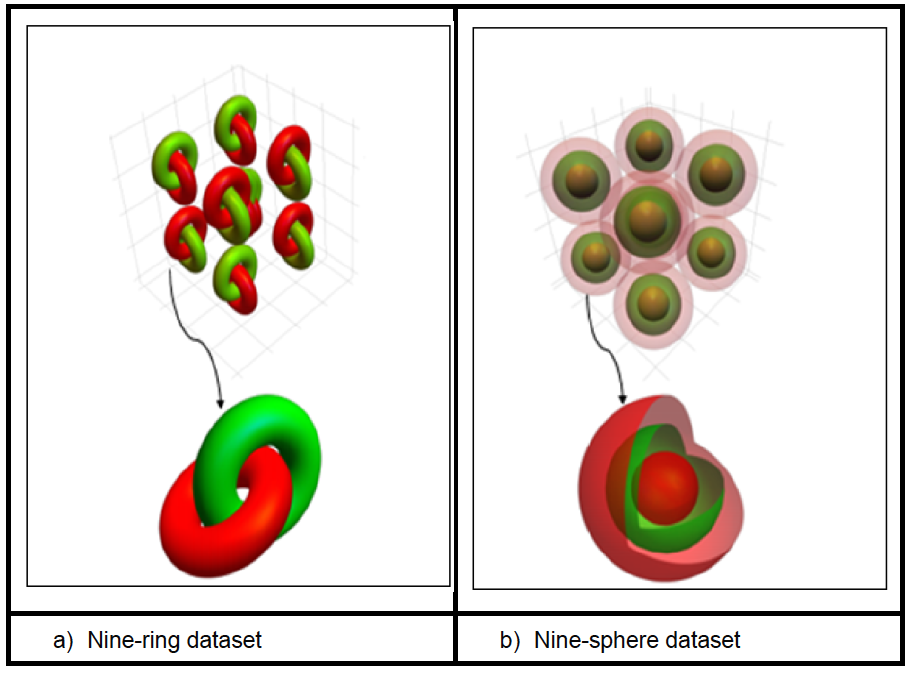
\includegraphics[width=0.8\textwidth]{images/nine_ring_and_nine_sphere.png}
\caption{3-dimensional synthetic datasets with two different classes(Red and Green) used for training MLP. \\ \footnotesize{Source: https://arxiv.org/abs/2004.06093}}
    \label{fig:nine_ring_and_nine_sphere}
\end{center}
\end{figure}

In addition, we also perform experiments and provide results on the following real datasets:
\begin{enumerate}
\item Cat-Dog dataset in Kaggle -- The dataset consists of  images of size $32 \times 32$. The dataset is divided into training and testing sets, with 8000 training images and 2000 testing images,  each set with an equal number of images of cats and dogs.
\item Fashion MNIST -- The dataset consists of 70,000 grayscale images of size $28 \times 28$ with 10 different categories. The dataset is divided into training and testing sets, with 60,000 training images and 10,000 test images.
\item CIFAR-10 -- The dataset consists of 60,000 colour images of size $32 \times 32$ with 10 different categories. Each category consists of 6000 images. The dataset is divided into training and testing sets, with 50,000 training images and 10,000 test images.
\end{enumerate}

Sample images from each of the above datasets are shown in Figures \ref{fig:catdog},  \ref{fig:fashionmnist}  and  \ref{fig:cifar10}. The datasets were converted to gray scale and normalized. No other preprocessing was performed.

\begin{figure}[htp]
\begin{center}
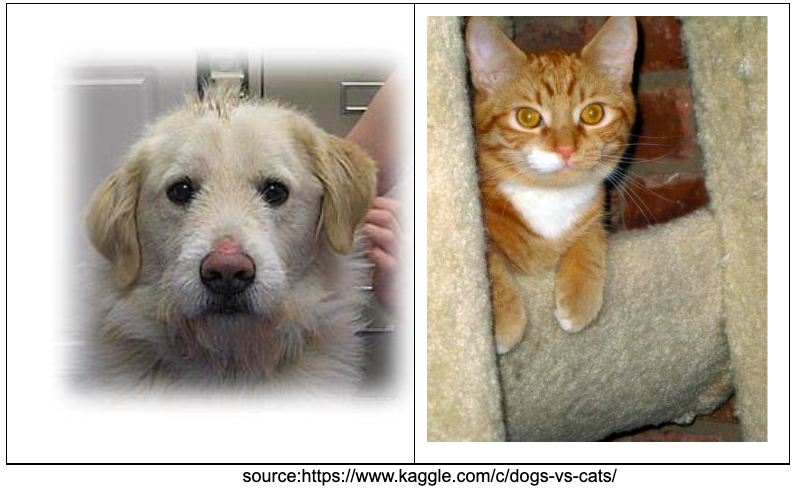
\includegraphics[width=0.8\textwidth]{images/catdog.png}
\caption{Sample images from Cat-Dog dataset}\label{fig:catdog}
\end{center}
\end{figure}

\begin{figure}[htp]
\begin{center}
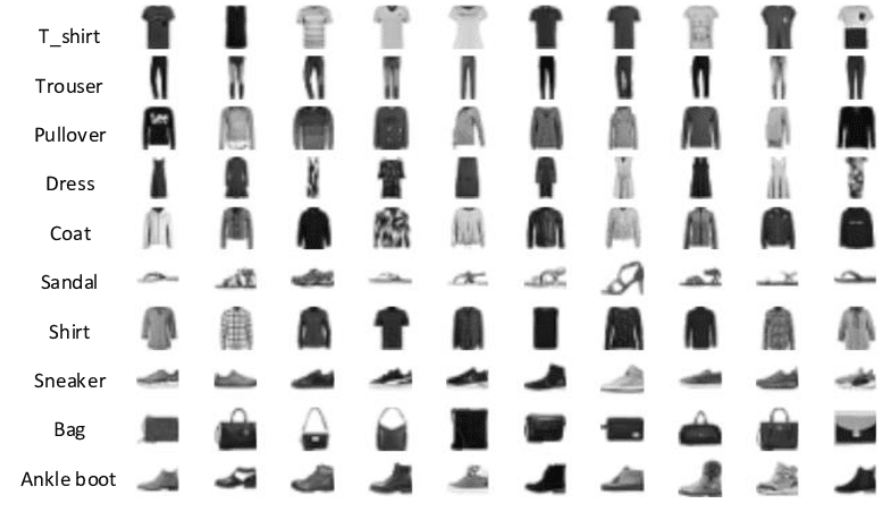
\includegraphics[width=0.8\textwidth]{images/fashionmnist.png}
\caption{Sample images from each of the 10 categories in Fashion MNIST dataset.}\label{fig:fashionmnist}
\end{center}
\end{figure}

\begin{figure}[htp]
\begin{center}
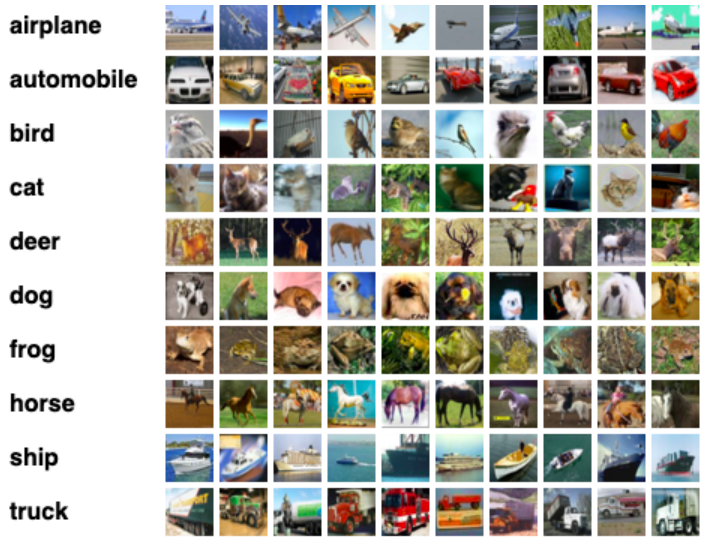
\includegraphics[width=0.8\textwidth]{images/Cifar10.png}
\caption{Sample images from CIFAR-10 dataset}\label{fig:cifar10}
\end{center}
\end{figure}

\subsection{Layer Transfer Function}
The layer transfer function is composed of an affine transformation and a non-linear activation function. The generic form of layer transfer function in MLP and CNN is given in Equations \ref{eq:1} and \ref{eq:2} below.

\begin{equation} \label{eq:1}
  X^{l + 1} = f(W^TX^{l} + b)
\end{equation}
where:
\begin{align*}
X^{l + 1} &= \text{Output of layer $l + 1$ }\\
X^{l} &= \text{Output of layer $l$} \\
W &= \text{Weight matrix} \\
b &= \text{Bias vector and} \\
f(.) &: \text{Non-linear activation function}\\
\end{align*}

\begin{equation} \label{eq:2}
  x_{ij}^{l + 1} = f(\sum_{m,n \in N(i,j)}{w_{mn}x_{mn}^{l} + b)}
\end{equation}
where:
\begin{align*}
x_{ij}^{l + 1} &= \text{Output value of layer $l + 1$ at pixel location $(i,j)$ }\\
N(i,j) &= \text{Set of pixels in a square nieghbourhood centered at pixel $(i,j)$.} \\
w_{mn} &= \text{Convolutional filter weights } \\
b &= \text{Bias }
\end{align*}

In the subsections below, we provide the details of desired characteristics for activation function from a topological point of view.

\subsection{Significance of Betti numbers on  layer transfer function}
Betti numbers, denoted as $\beta_k(X)$,   are used to quantify the topological complexity of a $d$-dimensional topological space  $X$, where  $0 \leq k \leq d-1$. The  $0^{th}$ Betty number, $\beta_0(X)$, is the number of connected components, the first Betti number, $\beta_1(X)$, is the number of one dimensional holes, the second Betti number, $\beta_2(X)$, is the number of two dimensional holes and so on. Figure \ref{fig:bett_numbers_illustration} shows some topological spaces and their corresponding Betti numbers.

\begin{figure}[htp]
\begin{center}
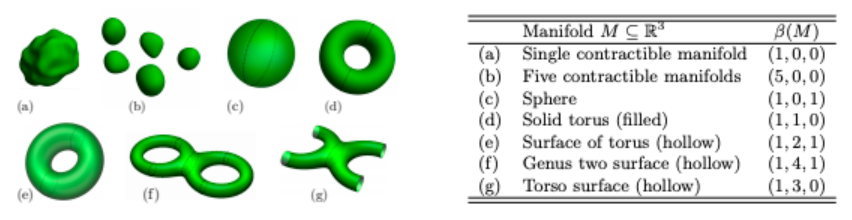
\includegraphics[width=0.8\textwidth]{images/bett_numbers_illustration.png}
\caption{Examples of some complex topological spaces and corresponding Betti numbers.\\ \footnotesize{Source: https://arxiv.org/abs/2004.06093}}
\label{fig:bett_numbers_illustration}
\end{center}
\end{figure}

For efficient classification, one needs to transform the original point data cloud, $X$,  from a high dimensional space with large Betti numbers to a low dimensional latent representation with  $\beta_0(X)$ (number of connected components) equal to the number of classes $K$ and all other Betti numbers to zero. As evident from Figure \ref{fig:topological_simplication_layer_by_layer} , this ensures that each connected component  corresponds to a single class (either Red or Green) and there are no holes within the connected components. Hence  each connected component is contractible  to a single point. It is easy to find a decision boundary if there are no holes on the manifold formed by samples from a  single class.

\begin{figure}[htp]
\begin{center}
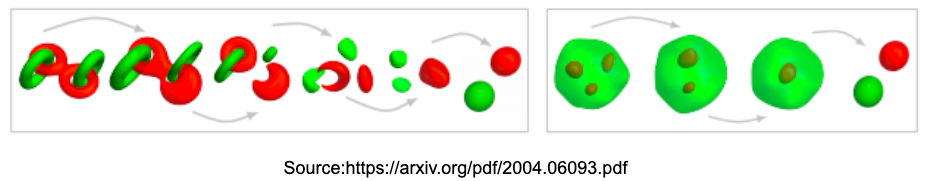
\includegraphics[width=0.8\textwidth]{images/topological_simplication_layer_by_layer.png}
\caption{Simplification of topological space as the data is transformed by successive layers of neural network.
}\label{fig:topological_simplication_layer_by_layer}
\end{center}
\end{figure}

\subsection{Design of activation function} \label{sec:design_of_activation_function}
It is observed that non-homeomorphic activation functions like ReLU reduce the Betti numbers faster as opposed to traditional  activation functions like sigmoid and tanh which are  homeomorphic Naitzat et al. (2020). Further, the more the number of discontinuities, the more powerful the activation function will be in terms of reducing the topological complexity. In addition to these findings, we also hypothesize that multiple many-to-one regions in the layer transfer function can reduce the topological complexity  of samples within a single class, as it tries to bring more samples together. As shown in Figure \ref{fig:activation_function_design}, we start with  a portion of a single half cycle of a sine function, and select a cut-off point $x=\frac{3\pi}{4}$. The selected portion of the sine function is repeated to get the final activation function as shown in the last figure in Figure \ref{fig:activation_function_design}.

\begin{figure}[htp]
\begin{center}
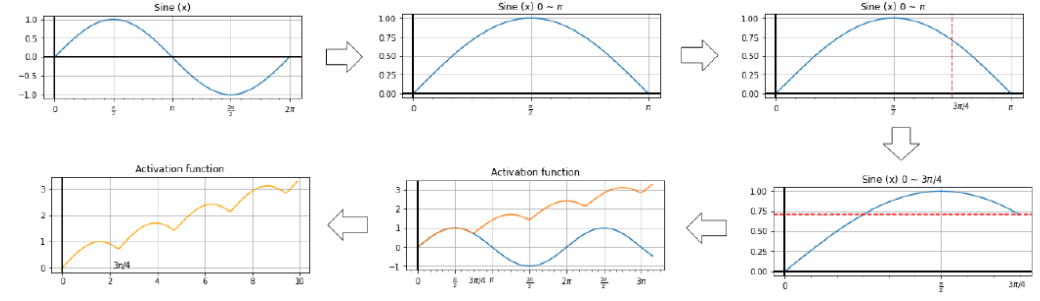
\includegraphics[width=0.8\textwidth]{images/activation_function_design.png}
\caption{Steps in design of many-to-one activation functions. We start with a single half cycle of a sinusoidal function an decide a cutoff-point $\frac{3\pi}{4}$ and repeat the function in the interval $[0,\frac{3\pi}{4}]$ to get the final activation function.}
\label{fig:activation_function_design}
\end{center}
\end{figure}

The final analytical form of activation function is
\begin{equation}
y = ksin(\frac{3\pi}{4})   + sin(x - \frac{3\pi}{4})
\end{equation}
 where $k=\left \lfloor{\frac{x}{\frac{3\pi}{4}}}\right \rfloor$

\subsection{Neural Network Architecture}
We performed experiments using MLP  on nine-sphere and nine-rings datasets. For image datasets, we used Convolutional Neural Networks for running the experiments. The MLP for simulated dataset consists of 9 layers with 25 neurons in each layer. We performed experiments with LeakyReLU and the proposed activation function. Our empirical results show that the proposed activation function results in faster training convergence compared to LeakyRelu.

\section{Results and Discussion}

\begin{figure}[htp]
\begin{center}
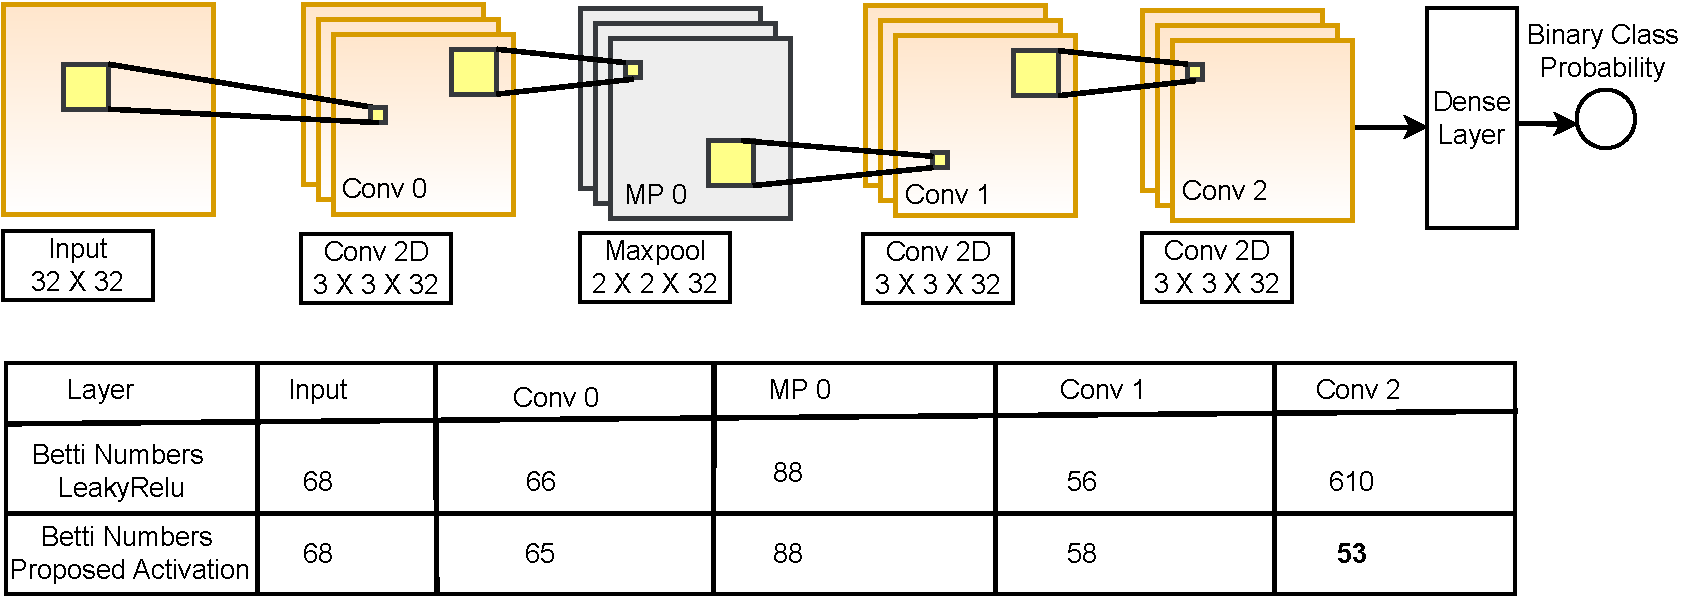
\includegraphics[width=0.8\textwidth]{images/cifar_10_arch.drawio}
\caption{Architecture of CNN for classifying images in CIFAR-10 dataset along with the comparison  of progression of first Betti number (Number of connected components) of samples from a single class across the layers using ReLU  and proposed activation function. First row of the table shows Betti numbers using LeakyReLU. Second row shows the Betti numbers with the proposed activation function added in layer Conv 2. It is observed that Betti number reduce significantly in layer Conv 2.
}
\label{fig:cifar_10_arch}
\end{center}
\end{figure}


Figure \ref{fig:cifar_10_arch} shows  comparison of progression of first Betti numbers (number of connected components) as the data is trasnformed across layers when Leaky ReLU is is used in all the layers Vs the proposed activation function is used is the final convolutional layer.  It is observed, from Figures \ref{fig:cifar_10_arch},  that with the proposed activation function Betti numbers decrease  by a significantly larger amount than ReLU activation function. Figure \ref{fig:training_convergence} shows the comparison of convergence  of multi layer perceptron with ReLU and proposed activation function using nine-sphere and nine-ring datasets. As evident from this figure, the reduction in Betti numbers  directly translates to faster training convergence. The new activation functions with multiple many-to-one regions seem to work well on various datasets and help in achieving at-par or better trainability.

\begin{figure}[htp]
\begin{center}
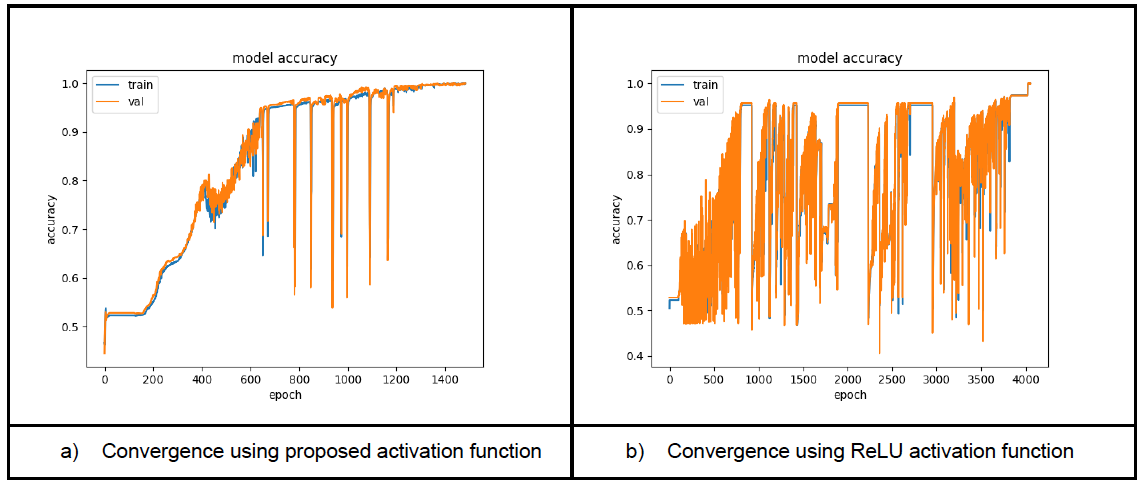
\includegraphics[width=0.8\textwidth]{images/training_convergence.png}
\caption{Architecture of CNN for classifying images in CIFAR-10 dataset along with the comparison  of progression of first Betti number (Number of connected components) of samples from a single class across the layers using ReLU  and proposed activation function. First row of the table shows Betti numbers using LeakyReLU. Second row shows the Betti numbers with the proposed activation function added in layer Conv 2. It is observed that Betti number reduce significantly in layer Conv 2.}
\label{fig:training_convergence}
\end{center}
\end{figure}

Also, The performance impact becomes more pronounced at larger batch-sizes i.e. with larger batch-sizes the gain tends to reach a factor of 2. On increasing the batch size the training for even simpler datasets takes longer (more epochs) for legacy activation functions. Even though the increase in training epochs  is seen for the proposed activation function also, the increase is less pronounced.

We further observed that,  in contrast to legacy activation functions like LeakyRelu,  the need to adjust learning rate seems to be little.

\section{Conclusion}
In this work, we look at topological complexity of data at the output of each layer of deep neural network for binary classification tasks. We propose a new activation function that simplifies the topological complexity of point cloud data (measured using Betti numbers)  at each hidden layer which translates to faster training convergence. We evaluate the proposed methods on popular image classification datasets and our results show 1) the proposed activation function results in faster training convergence and 2) removing hidden channels with large Betti numbers does not reduce the test accuracy which indicates that these feature maps are insignificant and can be removed.

%\acks{Acknowledgements should go at the end, before appendices and references. You can uncomment this for the camera-ready version on paper acceptance.}

%\bibliographystyle{plain}
\bibliography{acml22}

%\appendix
%
%\section{First Appendix}\label{apd:first}
%
%This is the first appendix.
%
%\section{Second Appendix}\label{apd:second}
%
%This is the second appendix.


\end{document}
